\chapter{Implementation}
\label{chap:implementation}

\section*{}
Here be dragons.

\section{Map generation and retrieval}
\label{section:map-generation}

To simulate the waste generation and collection, there is the need to provide a
topological city map. This topological map must be represented as a directed
weighted graph, so that routing algorithms may be applied. Being that a city is
usually a sparse graph, I opted for a adjacency list representation. To obtain
the maps, two different approaches were implemented.

First, I implemented the generation of random cities based on the official
RoboCup Rescue simulator. This procedure is detailed in
Section~\ref{section:roborescue}.

I also developed a more realistic approach, described in
Section~\ref{section:osm}  --- a procedure which allows the importation of city
maps from OpenStreetMap.org.




\subsection{RoboCup Rescue Random City Generation}
\label{section:roborescue}

RoboCup Rescue is a competition in which the participants must build agents to
control robot rescue teams, aiming to save the maximum number of people in a
city, after a catastrophe, such as an earthquake. This competition also
requires a city graph, so that the rescue vehicles can navigate through it.
The official simulator contains a procedure for the generation of random
cities, which is described by Teutenberg\citep{Teutenberg03}. Next, it is
presented a short description of this procedure:

\begin{enumerate}
	\item generate a uniformly distributed rectangular grid
	\item randomly shift each intersection in both axis
	\item remove random roads
	\item subdivide overlapping roads, by creating new intersections
	\item weight the roads, according to their usage based on a random set of paths
	\item smooth main roads
\end{enumerate}

As noted in the User's guide, the fourth step implementation is not correctly
implemented. This, along with other references to implementation problems, led
us to write the generator from scratch.

To implement the road intersection removal, there is a widely known algorithm
by Bentley and Ottman\cite{bentley-ottman} whose running time --- $O((n + k)
log~n)$, with $n$ being the number of roads and $k$ the number of overlaps ---
is significantly lower than the naive technique of checking each pair of
segments, which runs in $O(n^2)$.

\begin{figure}[h]
\centering
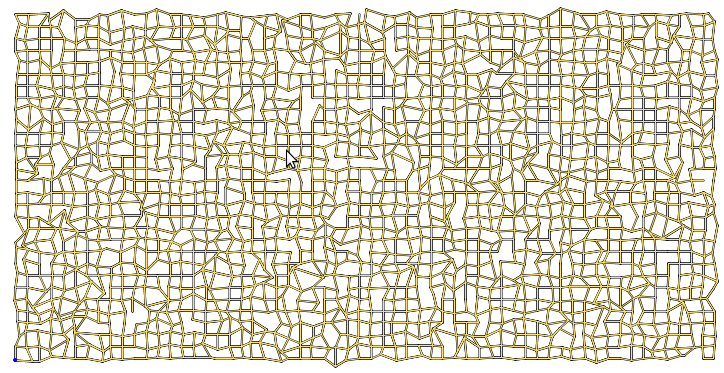
\includegraphics[width=0.75\textwidth]{random_map.png}
\caption{A random city map, generated using RoboCup Rescue official generator}
\label{fig:random_map}
\end{figure}

The maps obtained using this method, as seen in figure~\ref{fig:random_map},
have a grid-like topology. This trait gives them an unrealistic look, which may
be seen as a disadvantage. Regardless of this, maps obtained using this method
may be useful. By tweaking the procedure's parameters, one can obtain city maps
very different from each other, such as the one in
figure~\ref{fig:chaotic_map}. This may be used an easy way to generate
scenarios in which different routing algorithms can be applied, benchmarked and
compared.

\begin{figure}[h]
\centering
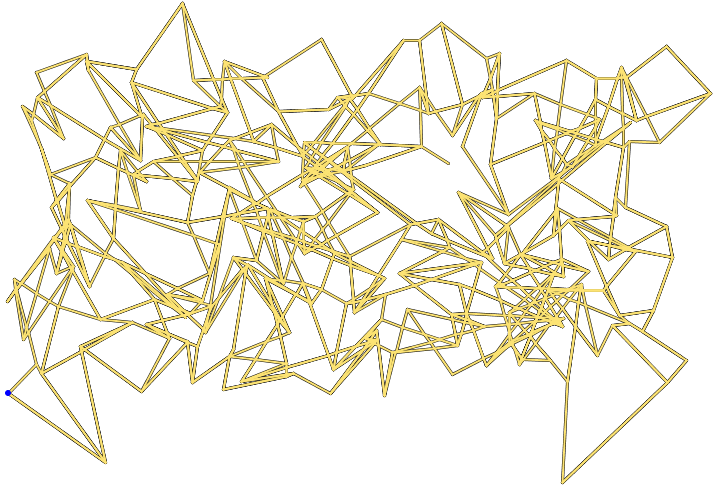
\includegraphics[width=0.75\textwidth]{chaotic_map.png}
\caption{By tweaking parameters of the RoboCup Rescue procedure, different maps can be obtained}
\label{fig:chaotic_map}
\end{figure}




\subsection{\osm{} Data Retrieval}
\label{section:osm}

Random maps may be used for simulation and benchmarking purposes, but there's
also the need to obtain real city maps. In order to obtain this information, an
application that imports maps from \osm{} --- whose data are free for use ---
was developed.  In figure~\ref{fig:porto} we present an example of a city
imported from \osm{}.

\begin{figure}[th]
  \begin{center}
    \leavevmode
    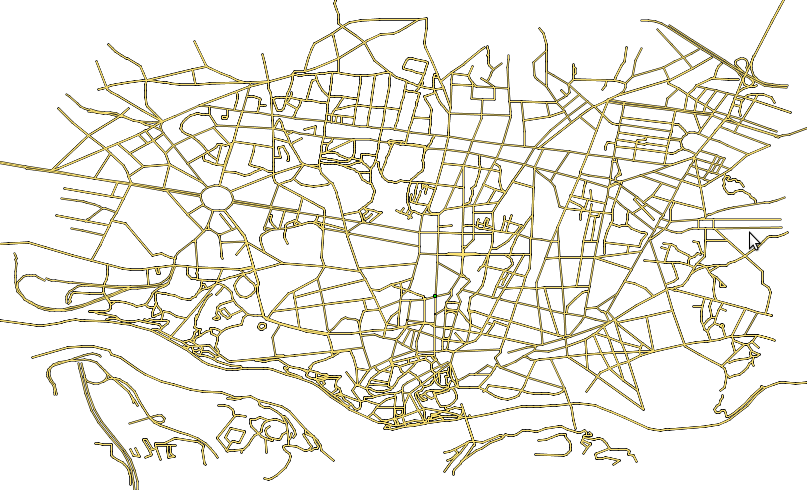
\includegraphics[width=0.75\textwidth]{porto}
    \caption{The city of Porto, Portugal, retrieved from \osm{} and loaded onto the current framework viewer.}
    \label{fig:porto}
  \end{center}
\end{figure}





\subsection{Stochastic waste generation parameters}
\label{section:parameters}

Each containers' fill rate varies according to several parameters, such as the
population density of the surrounding blocks, the socioeconomic level, the time
of the year and the area type --- residential, commercial or industrial, for
example. These topics were studied by Gómez et al, regarding the city of
Chihuahua, México in 2006\citep{Gomez20092018,Gomez20082465}.

As the correlation between these parameters and the waste generation rate is
not yet established (due to the lack of a fill status monitoring system), they
must be estimated. This can be done using the population density of the city
and data on kilograms per capita per day.





